% \begin{frame}{Modelagem}
%     \begin{itemize}
%         \item Qual problema estamos tentando resolver?
%     \end{itemize}
% \end{frame}

\begin{frame}{Modelagem - Recursos}
    \begin{columns}[T]
        \begin{column}{.5\textwidth}
            Recursos:
            \begin{itemize}
                \item Infraestrutura da rede.
                \item Comunicação entre recursos.
                \item Grafo.
            \end{itemize}
        \end{column}

        \begin{column}{.5\textwidth}
            \begin{figure}
                \centering
                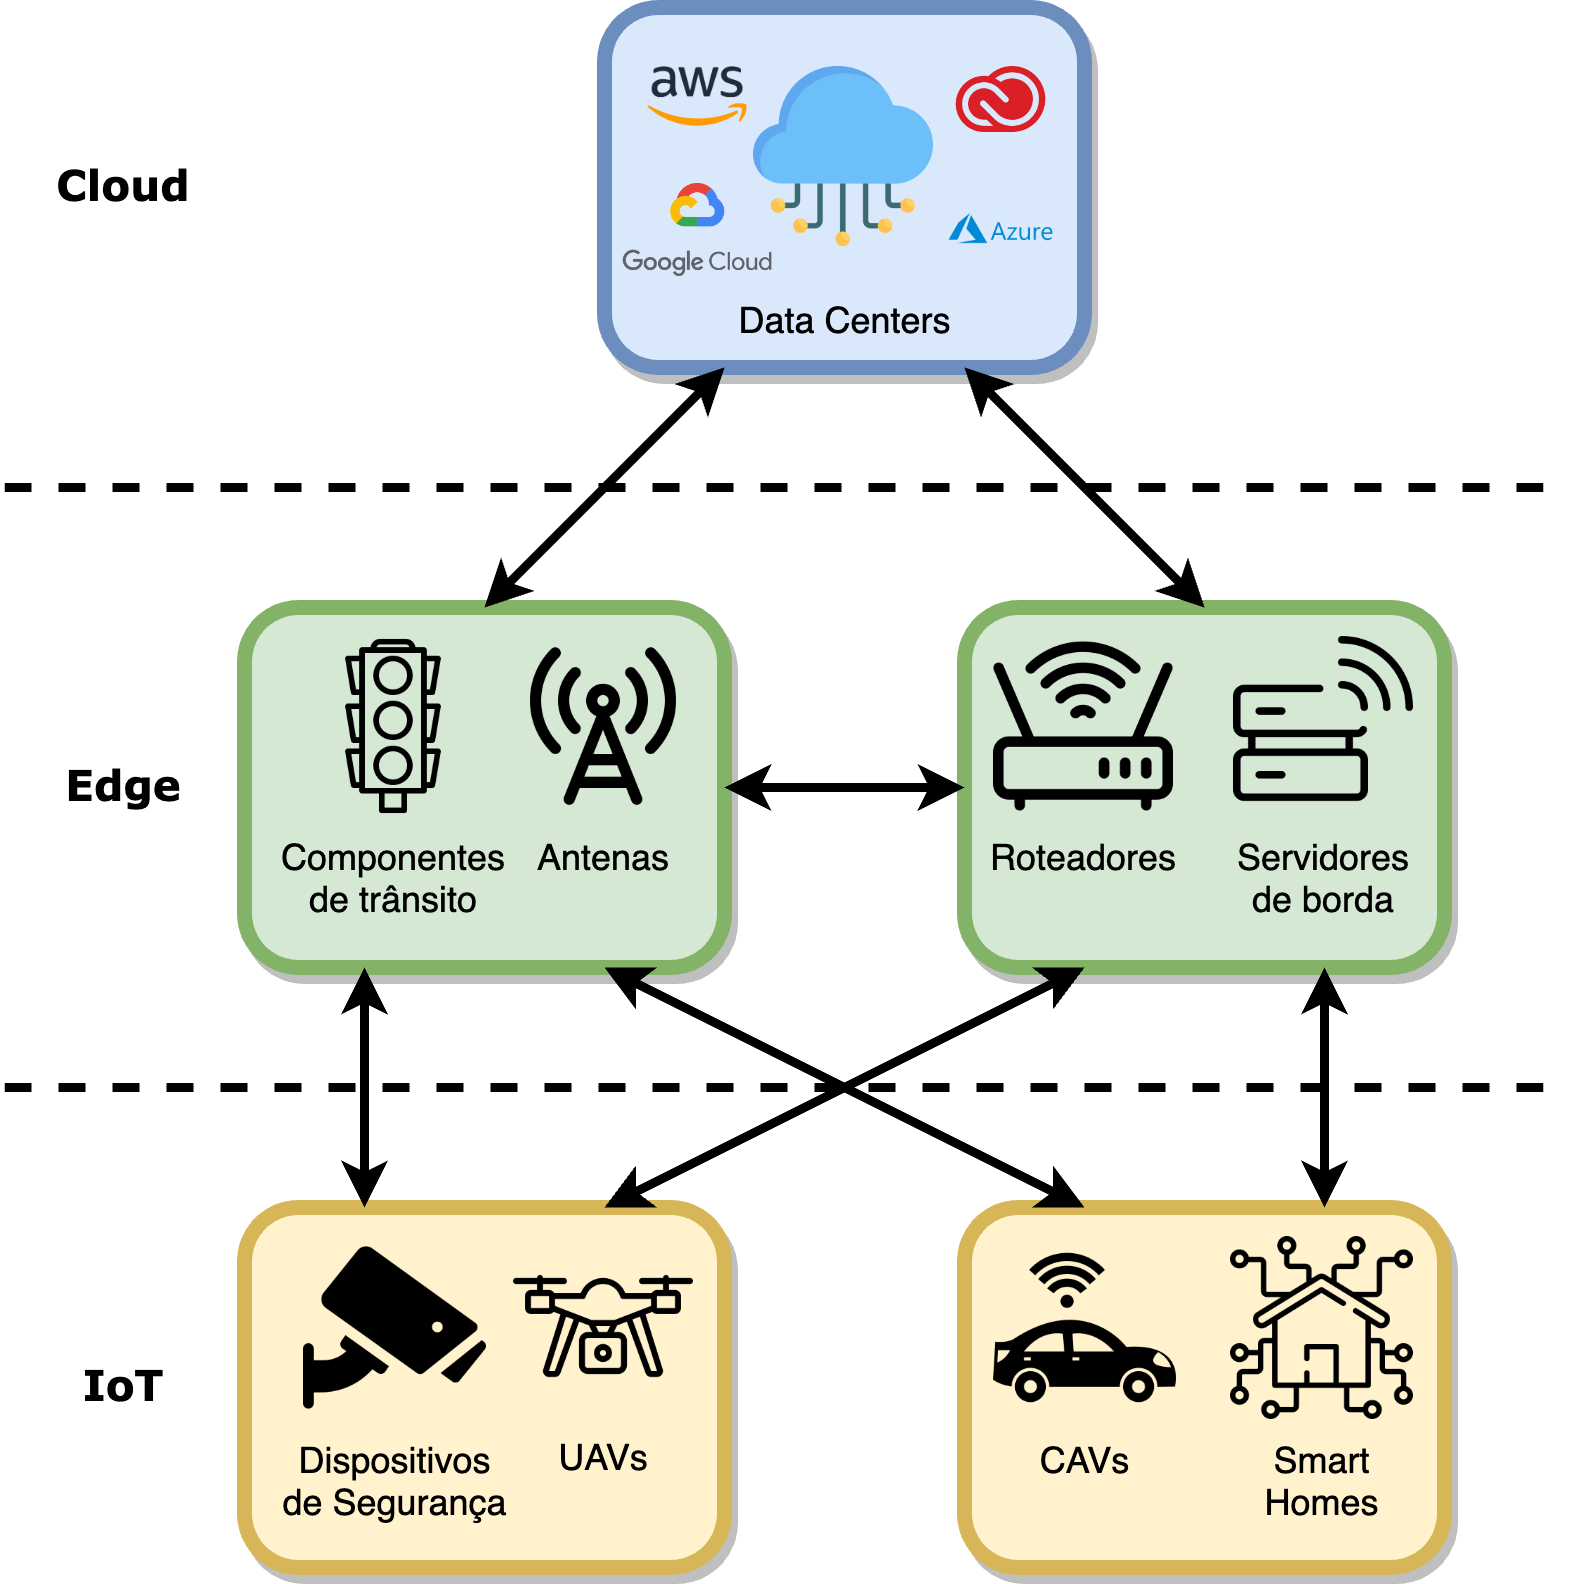
\includegraphics[width=\textwidth]{Figuras/TCC Edge Cloud IoT.png}
            \end{figure}
        \end{column}
    \end{columns}
\end{frame}

\begin{frame}{Modelagem - Tarefas}
    \begin{columns}[T]
        \begin{column}{.5\textwidth}
            Tarefas:
            \begin{itemize}
                \item Dados.
                \item Dependências de tarefas.
                \item Grafo acíclico e direcionado.
            \end{itemize}
        \end{column}

        \begin{column}{.5\textwidth}
            \begin{figure}
                \centering
                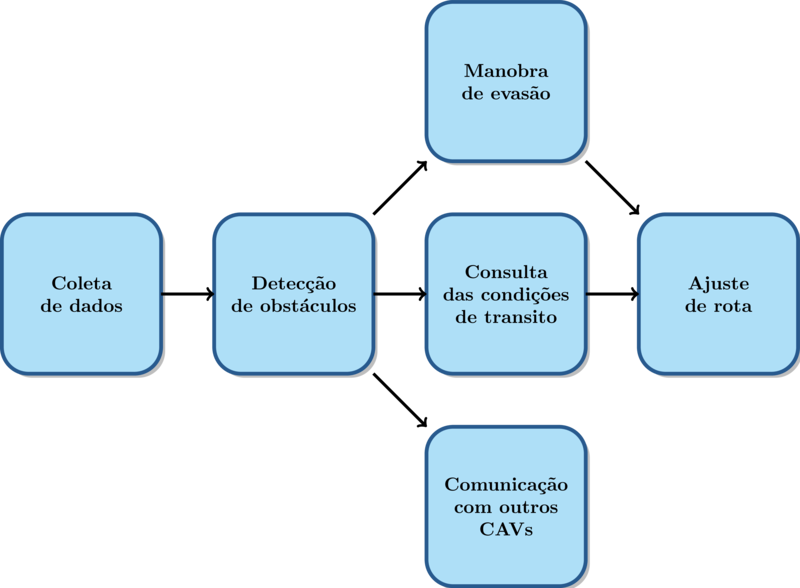
\includegraphics[width=\textwidth]{Figuras/cav-task.png}
            \end{figure}
        \end{column}
    \end{columns}
\end{frame}

\begin{frame}{Modelagem - Escalonamento}
    Escalonamento:
    \begin{itemize}
        \item Atribuir e ordenar tarefas a recursos.
        \item Entrada:
        \begin{itemize}
            \item[--] Grafo de recursos.
            \item[--] DAG de tarefas.
        \end{itemize}
        \item Saída:
        \begin{itemize}
            \item[--] Sequencia de mapeamentos de tarefas para recursos.
        \end{itemize}
        \item Otimizar Política de escalonamento:
        \begin{itemize}
            \item[--] Minimizar tempo de processamento.
            \item[--] Minimizar consumo de energia.
        \end{itemize}
    \end{itemize}
\end{frame}